\noindent Some Identities:\par
Ward Identity:
\[k_\mu M^{\mu}=0\]\par
Gordon Identity:
\[\bar{u}(p')\gamma^\mu u(p)=\bar{u}(p')\{\frac{p'^\mu+p^\mu}{2m}+\frac{i\sigma^{\mu\nu}q_\nu}{2m}\}u(p)\]
\subsection{Soft Bremsstrahlung}
The Current for a arbitory trajectory $y^\mu(\tau)$ is:
\[j^\mu(x)=e\int d\tau \frac{dy^\mu(\tau)}{d\tau}\delta^(4)(x-y(\tau))\]
we can consider a eletron with p get a sudden kick at$ (0,\vec{0})$ which illustrated in figure \ref{fig:soft}
\begin{figure}
\begin{center}
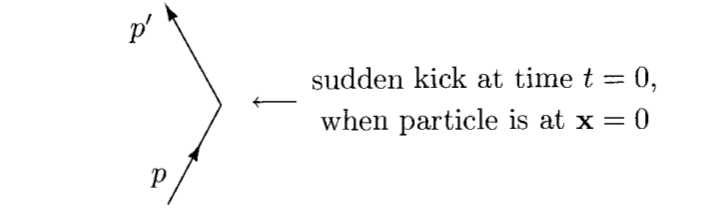
\includegraphics[height=4cm]{./figures/soft}
\caption{Soft Bremsstrahlung case: a electron get a sudden kick.}
\label{fig:soft}
\end{center}
\end{figure}
for this process, we can use the current as a source to solve the maxwell equation to get the potential:
\[A^{\mu}(x)=\int \frac{d^4k}{(2\pi)^4}e^{-ikx}\frac{-ie^2}{k^2}(\frac{p'^\mu}{p\bullet k'+i\epsilon}-\frac{p^\mu}{p\bullet k-i\epsilon})\]
and the riadiative part of the potential is:
\[A^\mu_rad(x)=Re\int \frac{d^3k}{(2\pi)^3}e^{-ikx}A^\mu(k)\]
where:
\[A^\mu(k)=\frac{-e}{|\vec{k}|}(\frac{p'^\mu}{p\bullet k'+i\epsilon}-\frac{p^\mu}{p\bullet k-i\epsilon})\]
and the energy radiatied is:
\[E=\int \frac{d^3k}{(2\pi)^3}\sum_{\lambda=1,2}\frac{e^2}{2}(\frac{2p\bullet p'}{(k\bullet p')(k\bullet p)}-\frac{m^2}{(k\bullet p')^2}-\frac{m^2}{(k\bullet p)^2})\]
Calculating the same quantity using quantum theory:
\[d\sigma(p\rightarrow p'+\gamma)=d\sigma(p\rightarrow p')\int \frac{d^3k}{(2\pi)^3}\frac{1}{2k}\sum_{\lambda=1,2}e^2|\epsilon_\lambda\bullet(\frac{p'}{p'\bullet k}-\frac{p}{p\bullet k})|^2\]
\[d\sigma(p\rightarrow p'+\gamma)=_{-q^2\rightarrow \infty}d\sigma(p\rightarrow p')\frac{\alpha}{\pi}\ln(\frac{-q^2}{\mu^2})\ln(\frac{-q^2}{m^2})\]
where $\mu$ is assumed tiny mass for photon to solve the divergence.\par
\subsection{The Electron Vetex Function}
Just as the figure \ref{fig:vertex} shows,we suppose the vertex is:
\[-ie\Gamma^\mu(p',p)\] 
\begin{figure}
\begin{center}
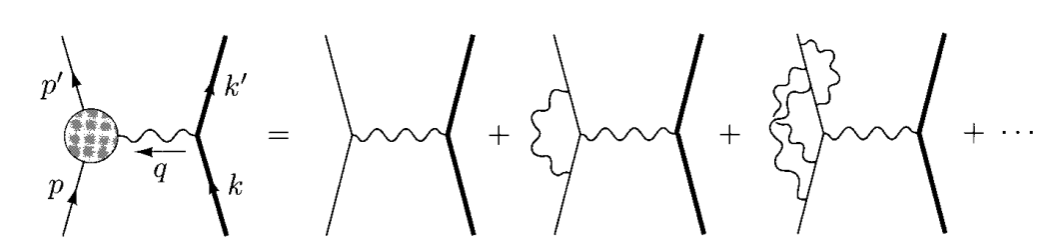
\includegraphics[height=4cm]{figures/vertex}
\caption{Electron Vertex Structure Illustration}
\label{fig:vertex}
\end{center}
\end{figure}
Using the Lorentz Invariance and Ward identity we can get the general form for it:
\[\Gamma^\mu(p',p)=\gamma^\mu F_1(q^2)+\frac{i\sigma^{\mu\nu}q_\nu}{2m}F_2(q^2)\]
where $F_1$ and $F_2$ is unkown function called \textcolor{red}{form factor}\par
for the Lande g-factor we have the ralation:
\[g=2(F_1(0)+F_2(0))\]
A trick for some integration:
\[\frac{1}{A_1A_2\cdots A_n}=\int_0^1dx_1\cdots dx_n\delta(\sum x_i-1)\frac{(n-1)!}{(x_1A_1+\cdots x_n A_n)^n}\]
\[\frac{1}{A_1^{m_1}A_1^{m_2}\cdots A_n^{m_n}}=\int_0^1dx_1\cdots dx_n\delta(\sum x_i-1)\frac{\prod x_i^{m_i-1}}{(\sum x_i A_i)^{\sum m_i}}\frac{\Gamma(m_1+\cdots m_n)}{\Gamma(m_1)\Gamma(m_2)\cdots\Gamma(m_n)}\]
\textcolor{red}{Feymann Parameter}:\par
\begin{align*}
\frac{1}{(k-p)^2(k^2-m^2)}&=\int_0^1 dxdy\delta(x+y-1)\frac{1}{[x(k-p)^2+y(k^2-m^2)]^2}\\
&=\int_0^1 dxdy\delta(x+y-1)\frac{1}{(k^2-2xk\cdot p+xp^2-ym^2)^2}
\end{align*}
when we define $l=k-xp$, then the whole integration is only rely on the $l^2$ and can trasfer to spherical coordinate to calculate the monmentum integration.the variable x,y is called Feymann Parameter.\par
we can use Wick rotation to change from Minkovski space to Eculid Space:
\[l^0=il_E^0;\hspace{3em} \vec{l}=\vec{l}_E\] 
then the intergration becomes:
\[\int d^4l\frac{1}{(l^2-\Delta)^m}=\frac{i}{(-1)^m}\frac{1}{(2\pi)^4}\int d^4l_E\frac{1}{(l_E^2+\Delta)^m}\]
the right hand side inner product of the above equation is the inner product in Eculid Space.
Using all the tricks above ,one can work out the diagram(figure \ref{fig:vertexcal}):
\begin{figure}
\begin{center}
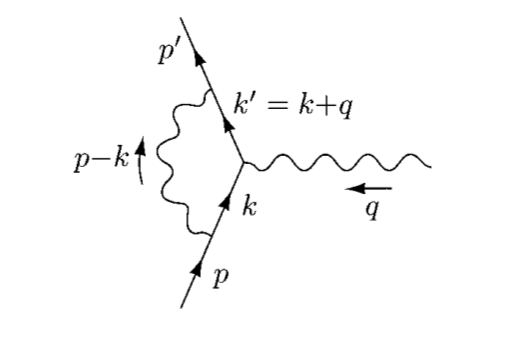
\includegraphics[height=4cm]{figures/vertexcal}
\caption{the order-$\alpha$ for $\Gamma^\mu$}
\label{fig:vertexcal}
\end{center}
\end{figure}
\begin{align*}
&\frac{\alpha}{2\pi}\int^1_0dxdydz\delta(x+y+z-1)\\
&\times \bar{u}(p')(\gamma^\mu[\ln\frac{z\Lambda^2}{\Delta}+\frac{1}{\Delta}((1-x)(1-y)q^2+(1-4z+z^2)m^2)]\\
&+\frac{i\sigma^{\mu\nu}q_\nu}{2m}[\frac{1}{\Delta}2m^2z(1-z)])u(p)
\end{align*}
where $\Lambda$ is a Parameter Introduced to solve the divergence.:
\[\frac{1}{(k-p^2)+i\epsilon}\rightarrow_{\Lambda\rightarrow \infty} \frac{1}{(k-p^2)+i\epsilon}-\frac{1}{(k-p^2)-\Lambda^2+i\epsilon}\]
with such substraction,the divergence of this type:
\[\int dl^2\frac{l^4}{(l^2+\Delta)^3}\rightarrow\int dl^2(\frac{l^4}{(l^2+\Delta)^3}-\frac{l^4}{(l^2+\Delta_\Lambda)^3})\]
\subsection{Summution And Interpreatation of Infrared Divergence.}
\begin{figure}
\begin{center}
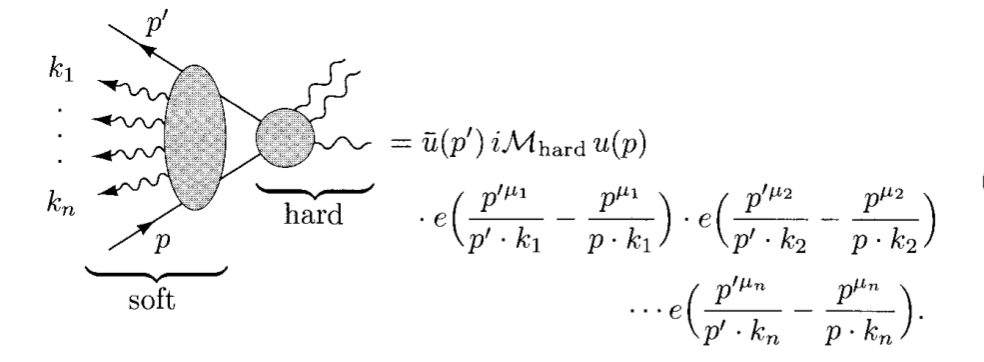
\includegraphics[height=4cm]{figures/VertexForm}
\caption{One can work out such diagram}
\end{center}
\end{figure}
and for a vitural photon such as the diagram like figure \ref{fig:vertexcal},Its value is(when connected to another diagram):
\[\frac{e^2}{2}\int \frac{d^4 k}{(2\pi)^4}\frac{-i}{k^2+i\epsilon}(\frac{p'}{p'\cdot k}-\frac{p}{p\cdot k})(\frac{p'}{-p'\cdot k}-\frac{p}{-p\cdot k})=X\]
with above calculation :
\[X=-\frac{\alpha}{2\pi}f_{IR}(q^2)\ln\frac{-q^2}{\mu^2}\]
\begin{figure}
\begin{center}
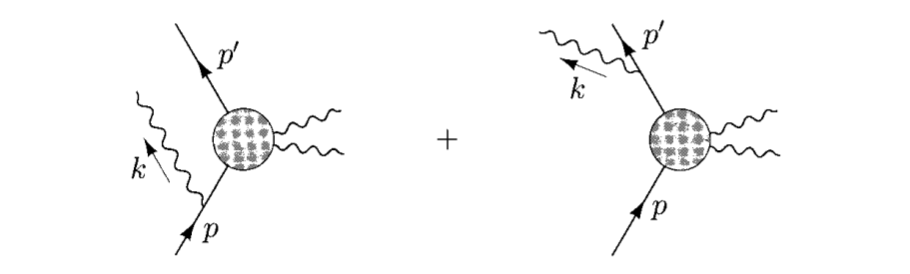
\includegraphics[height=4cm]{figures/realphoton}
\caption{scattering a real photon process}
\label{fig:realphoton}
\end{center}
\end{figure}
and the differential cross section for scattering a real photon like diagram(figure \ref{fig:realphoton}) is:
\[\int \frac{d^3k}{(2\pi)^3} \frac{1}{2k}(-g_{\mu\nu})(\frac{p'^\mu}{p'\cdot k}-\frac{p^\mu}{p\cdot k})(\frac{p'^\nu}{p'\cdot k}-\frac{p^\nu}{p\cdot k})=Y\]
with above calculation,we have:
\[Y=\frac{\alpha}{\pi}f_{IR}(q^2)\ln\frac{E_l^2}{\mu^2}\]
so we have:
\[\sum_{n=0}^\infty\frac{d\sigma}{d\Omega}(p\rightarrow p'+n\gamma)=\frac{d\sigma}{d\Omega}(p\rightarrow p')e^Y\]
and the correction for arbitrary vitural photon is:
\[\sum^{\infty}_{n=0}\frac{1}{n!}X^n=e^{X}\]
so the total differential cross section obseverd is:
\begin{align*}
(\frac{d\sigma}{d\Omega})_{measured}&=\frac{d\sigma}{d\Omega}(p\rightarrow p')e^{2X}e^Y\\
&=\frac{d\sigma}{d\Omega}(p\rightarrow p')e^{-\frac{\alpha}{\pi}f_{IR}(q^2)\ln\frac{-q^2}{E_l^2}}
\end{align*}
\par
\begin{center}
\textcolor{red}{\large{Which Is Not Depend On The  Vitural Photon Mass $\mu$}}
\end{center}
